\header{
    \section{Un poil de cul sur ma savonette} \label{un-poil-de-cul-sur-ma-savonette}
    %
    
    \insertComment{Parole de Jean-Marie Bigard.}{}
}

\enluminure{4}{\href{https://www.youtube.com/watch?v=srXc3tKIEc4}{E}}{lle} avait mis dans mon blouson
\\Des rêves bleus et des frissons
\\Ma météo c'était ses yeux
\\Quand ils brillaient, on était deux
\\\\Elle a tout pris dans la maison
\\Mon coeur ma vie, mes boîtes de thon
\\Elle m'a laissé comme un adieu
\\Une chose d'elle qui frise un peu
\\\\\textbf{Refrain :}
\\Un poil de cul sur ma savonnette
\\Et ça pollue toute ma planète
\\Sous l'eau chaude il reste collé 
\\Alors du doigt il faut gratter
\\Et puis sous l'ongle aller chercher
\\Le poil de cul 
\\Sur ma savonnette
\\\\Elle avait d'la conversation
\\Autant qu'une part de reblochon
\\Mais elle jouait du casse-noisette
\\Bien mieux qu'Armstrong, de la trompette
\\\\On faisait dans la salle de bain
\\Des trucs sans se servir des mains
\\Il ne reste de nos baisers
\\Qu'un souvenir noir et frisé
\\\\(C'est vrai un poil de cul c'est dégueulasse, elle aurait chié sur ma
bosse à dents ce s'rait pas pire, d'autant plus que, entre nous...)
\breakpage
Chuis d'ordinaire plutôt gentil
\\Je donne ma ch'mise et je souris
\\J'ai même laissé mon meilleur pote
\\Un jour de pluie, chier dans mes bottes
\\On peut me dire que ch'uis un con
\\Et boire ma bière et mon picon
\\Mais elle a vraiment tout gâché
\\Quand j'ai vu qu'elle m'avait laissé
\bigskip
\bigskip
\begin{center}
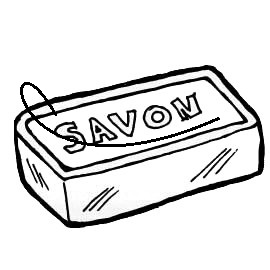
\includegraphics[width=1\textwidth]{images/savon.jpg}
\end{center}

\breakpage